
%% Version for one sided printing:
% margins: left 40mm, right 25mm, top and bottom 25mm
% (BUT LaTeX adds automaticly 1in)
\documentclass[12pt,a4paper]{report}
\setlength\textwidth{145mm}
\setlength\textheight{247mm}
\setlength\oddsidemargin{15mm}
\setlength\evensidemargin{15mm}
\setlength\topmargin{0mm}
\setlength\headsep{0mm}
\setlength\headheight{0mm}
% \openright makes following text start on right side of book
\let\openright=\clearpage

%% Version for two sided printing:
% \documentclass[12pt,a4paper,twoside,openright]{report}
% \setlength\textwidth{145mm}
% \setlength\textheight{247mm}
% \setlength\oddsidemargin{15mm}
% \setlength\evensidemargin{0mm}
% \setlength\topmargin{0mm}
% \setlength\headsep{0mm}
% \setlength\headheight{0mm}
% \let\openright=\cleardoublepage

%\usepackage[T1]{fontenc}
\usepackage[utf8]{inputenc}
%\usepackage[american]{babel}

\usepackage{comment}
\usepackage{setspace}

\usepackage{subfig}
\usepackage{wrapfig}
\usepackage{graphicx}
%\usepackage{amsthm}
\usepackage{booktabs}


\usepackage[autostyle]{csquotes}
\usepackage{xspace}

\usepackage[
	backend=biber,
	style=alphabetic,
	backref=true,
%	backrefstyle=all+,
	natbib=true,
	url=false, % url field of @online entries is always printed
	doi=false,
	eprint=false
]{biblatex}
\renewcommand{\labelalphaothers}{*}
\addbibresource{bibliography.bib}

\usepackage{color}
\definecolor{linkClr}{RGB}{127,0,0}  % dark red
\definecolor{citeClr}{RGB}{0,127,0}  % dark green
\definecolor{urlClr}{RGB}{0,0,127}  % dark blue

\usepackage{listings}  % \lstlisting enviroment - source code highliting

\usepackage{lsystemSyntax}  % uses packages color and listings

\usepackage[unicode]{hyperref}  % after all other packages
\hypersetup{
	pdftitle=L-systems online,
	pdfauthor=Marek Fišer,
	pdfkeywords={keyword1} {key2},
	colorlinks=true,
	linkcolor=linkClr,
	citecolor=citeClr,
	urlcolor=urlClr
}

%%% Little tweaks

% These macros remove white space above headers of chapters.
\makeatletter
\def\@makechapterhead#1{
  {\parindent \z@ \raggedright \normalfont
   \Huge\bfseries \thechapter. #1
   \par\nobreak
   \vskip 20\p@
}}
\def\@makeschapterhead#1{
  {\parindent \z@ \raggedright \normalfont
   \Huge\bfseries #1
   \par\nobreak
   \vskip 20\p@
}}
\makeatother

% Definition of chapter macro. Chapters are not numbered but they are in TOC.
\def\chapwithtoc#1{
\chapter*{#1}
\addcontentsline{toc}{chapter}{#1}
}

% default path for graphics
\graphicspath{{img/}}

% macros for L-system to avoid hyphenation of it.
\newcommand{\lsystem}{\mbox{L-system}\xspace}
\newcommand{\lsystems}{\mbox{L-systems}\xspace}

% for carons with t, d
\newcommand{\varcaron}{\hspace{-1.5pt}'\hspace{-1pt}}

\renewcommand{\ttdefault}{pcr}  % to allow bold in tt font

\newenvironment{itemize*}
	{\begin{itemize}
		%\setlength{\itemsep}{0pt}
		\setlength{\parskip}{0pt}}
	{\end{itemize}}
\newenvironment{enumerate*}
	{\begin{enumerate}\setlength{\parskip}{0pt}}
	{\end{enumerate}}

\widowpenalties 1 10000
\raggedbottom

\begin{document}

% A little freer hyphenation settings than the default.
%\lefthyphenmin=2
%\righthyphenmin=2

%
\pagestyle{empty}
\begin{center}

\large

Charles University in Prague

\medskip

Faculty of Mathematics and Physics

\vfill

{\bf\Large BACHELOR THESIS}

\vfill

\centerline{\mbox{\includegraphics[width=60mm]{logo}}}

\vfill
\vspace{5mm}

{\LARGE Marek Fišer}

\vspace{15mm}

% Name of thesis exactly according to the specification.
{\LARGE\bfseries L-systems online}

\vfill

% Official name of department or institute where the work was officially specified.
% (According to Internal Structure of MFF UK)
Department of Software and Computer Science Education

\vfill

\begin{tabular}{rl}

Supervisor of the bachelor thesis: & RNDr. Josef Pelikán \\
\noalign{\vspace{2mm}}
Study program: & Computer Science \\
\noalign{\vspace{2mm}}
Specialization: & Programming \\
\end{tabular}

\vfill

Prague 2012

\end{center}






































%%% Následuje vevázaný list -- kopie podepsaného "Zadání bakalářské práce".
%%% Toto zadání NENÍ součástí elektronické verze práce, nescanovat.

%
%%% At this point, can be written any thank (head work, literature, etc.)

\openright

\noindent
Dedication.










































%\include{affidavit}

\renewcommand{\lstlistingname}{Source code}



\section*{Abstrakt}

\mbox{L-systém} je v nejjednodušší podobě varianta bezkontextové gramatiky.
Byl vyvi\-nut a používá se hlavně pro modelování růstu rostlin, ale s jeho pomocí se také dají vytvářet obecné fraktály, modely měst nebo dokonce hudbu.
Pokud někoho \mbox{L-systémy} zaujmou a che s nimi experimentovat, je těžké najít aplikaci, která by mu to umožňovala.
Cílem této práce bylo vytvořit online systém, který by umožňoval práci a experimentování s L-systémy širokému spektru uživatelů.
Výsledné řešení se skládá ze dvou částí.

První část je univerzální, snadno rozšiřitelná knihovna pro zpracování \mbox{L-sys}\-témů.
Svou rozšiřitelnost dosahuje vysokou modularitou, vstup zpracovává pros\-třednic\-tvím systému propojených komponent, které jsou specializované na kon\-krét\-ní činnost.
To také přispívá k přehlednosti a spolehlivosti celku.
Navíc je knihovna zcela nezávislá a multiplatformní, lze ji tedy použít i v jiných aplikacích.

Druhá část je moderní webové rozhraní, které bylo navrženo tak, aby bylo srozumitelné pro nováčky a zároveň aby nabízelo pokročilé funkce pro nároč\-nější uživatele.
Pro vizualizaci 3D \mbox{L-systémů} využívá moderní technologie jako HTML5 WebGL.
Součástí webu je i galerie L-systémů do které může každý uživatel přispívat a tvořit tak komunitu.
Webové rozhraní plně využívá schopnosti navr\-žené knihovny a slouží tak i jako ukázka jejího použití.































\singlespacing
\openright
\pagestyle{plain}
\setcounter{page}{1}
\tableofcontents

\onehalfspacing

%
\chapwithtoc{Introduction}
\label{sec:Introduction}

An \lsystem (also called a Lindenmayer system) is a mathematical formalism that was developed by Aristid Lindenmayer in 1968 for modeling plant growth~\cite{Lin68}.
An example of a plant modeled by an \lsystem is shown in \autoref{fig:introLilac}.
In its simplest form an \lsystem is a variant of a regular or \mbox{context-free} grammar.
By rewriting (deriving) an initial string of symbols (also called an axiom) with some rewrite rules from a grammar, an \lsystem produces a new string of symbols which can be interpreted in many different ways.
In the first \lsystems by used Lindenmayer there symbols were to be interpreted as cells of algae.
Later, different approach was adopted by Przemyslaw Prusinkiewicz who interpreted the \lsystem symbols using \mbox{Logo-like} turtle drawing system%
	\footnote{Logo a is computer programming language developed for use in the education of programming for children.
	Logo controls a cybernetic turtle which does the drawing on a 2D canvas.}~\cite{Pru85}.
With this method he obtained more plant-like structures and fractals~\cite{CD93}.
In \autoref{fig:introHTree} you can see a H-tree fractal created by an \lsystem.

\begin{figure}[h!]
	\subfloat[Model of lilac panicle]{
		\includegraphics[width=0.49\linewidth]{lilac}
		\label{fig:introLilac}
	} \hfill
	\subfloat[H-tree fractal]{
		\includegraphics[width=0.49\linewidth]{HTree}
		\label{fig:introHTree}
	}
	\caption{Examples of models created by an \lsystem}
\end{figure}


Over time \lsystems began to used in many diverse areas.
For example they were used to generate rivers in fractal mountains~\cite{PH93}, streets in virtual cities~\cite{PM01} and to describe the subdivision of curves~\cite{PSSK03}.
\lsystems can be used in fields other than computer graphics: for example, in music generation~\cite{HCJ99, Man06}.
They are still used in plant modeling.
Plant models generated with \lsystems are used in modern video games or films: for example, they were used to generate many plants and trees for the famous film Avatar~\cite{Wor08, Dun10}.~\footnote{\citeauthor{SBM10} presented a reverse method -- the automatic generation of \lsystems from a 2D model~\cite{SBM10}.}

\lsystems have a wide variety of interesting applications but it is not easy to find a place to experiment with them.
Esentially there are two basic types of \lsystem generators: web-based and desktop applications.
Web-based \lsystem generators are easily accessible but they are often too primitive to offer much more than the generation of simple fractals (see \autoref{sec:WebBasedGenerators}).
Some of them do not even work in the most-used browsers.

Desktop applications generally offer more options than web-based ones but most of them are also quite simple and do not offer advanced types of \lsystems.
There are some complex applications that offer pretty good sets of features but these are expensive, not easy to control, and/or they are old and no longer maintained (see \autoref{sec:DesktopGenerators}).
A problem with desktop applications is also their compatibility with a user's operating system, its version, and the libraries installed.

The overall goal of this work is to take the best from both of the two main approaches and an create online, feature-rich, development environment for anybody who wants to experiment with \lsystems.
The development environment will be divided into two parts: a web user interface and an \lsystem processing library.

\begin{wrapfigure}{r}{0.5\textwidth}%
	\vspace{6pt}%
	\includegraphics[width=\linewidth]{MengerSponge}
	\caption{Menger sponge created by an \lsystem}
	\label{fig:introMengerSponge}
\end{wrapfigure}

The user interface will be web a site that offers great accessibility.
Anyone from around the world will be able to use it from any device connected to the Internet , such as: computers, laptops, tablets or smart phones.
The interface should be user-friendly to new users and also offer advanced features for experienced users.
The primary output format of the web-based \lsystem processor will be 2D images but it will also be possible to create and display 3D outputs using modern HTML5 WebGL%
	\footnote{WebGL (Web-based Graphics Library) is a cross-platform, royalty-free web standard for a low-level 3D graphics API based on OpenGL ES 2.0, exposed through the HTML5 Canvas element as Document Object Model interfaces.
		WebGL code executes on a computer display card's GPU (graphics processing unit).}
	technology directly in the browser.
In \autoref{fig:introMengerSponge} is a print-screen of a Menger Sponge model displayed by WebGL.
Part of the web site will be a gallery of \lsystems.
Any registered user can add his own \lsystems to the gallery along with a description and then others can rate it.
This will help to create a community of active users and it can also serve as a learning tool for new users.
\nomenclature{HTML5}{hypertext markup language}
\nomenclature{WebGL}{web graphics library}
\nomenclature{API}{application programming interface}
\nomenclature{GPU}{graphics processing unit}

The second part of the application will be the \lsystem processing library.
Although it will be designed to support the demands of a web interface, it will be independent and should be usable in other applications.
During the design of the library, great emphasis will be placed on its ease of extensibility to make it as universal as possible.
It should be possible to extend the library by the users themselves.

A new syntax for input will be designed to improve the user experience especially for new users.
The syntax should be clean, easy to understand and to remember.
%The syntax will cover all needs of library from defining \lsystems to configuring whole processing system.
%This will also ensure that whole input can be written in one file which will simplify source code sharing and saving.
%Parser generator will be used for creating robust and extensible parser.


\section*{Structure of the thesis}

In the first chapter a formal definition of \lsystems is given and principles for their rewriting and interpretation are explained.
Then follows some descriptions of \lsystem types and their properties.
At the end of the first chapter is a list of some related \lsystem generators.

The second chapter is devoted to the design of the solution.
There is described how \lsystem processing library and web user interface works.

Implementation details of the project are discussed in the third chapter.
Sections in this chapters explains individual problems and their solutions.
The text accompanies actual source code snippets and diagrams for better explanation.

The fourth chapter summarizes the results.
Part of this chapter is showcase of images of generated \lsystems.

All the source codes of \lsystems used in this thesis are in a syntax designed as a part of this work.
A reference to this syntax can be found in attachment \ref{chap:syntax}.
It is possible to process all the source code on the web.
More information about the figures in this thesis together with additional information and their source codes is given in attachment \ref{chap:aboutFigures}.

































%
\chapter{\lsystems}

A brief history of \lsystems has already been mentioned in the introduction.
In this chapter are \lsystems described more formally.
Follows explanation of the rewriting and interpretation principles of \lsystems.
The main focus of this chapter is to describe various \lsystem types.
At the end of the chapter is a list of related applications.



\section{Formal definition of \lsystem}

\lsystem $L$ is formally triplet $L = (\Sigma, \omega, R)$, where

\begin{itemize*}
	\item $\Sigma$ is \emph{alphabet}, non-empty set of symbols, $\Sigma^{*}$ is set of all words\footnote{Word is a sequence of symbols.} which can be created from the alphabet $\Sigma$, $\Sigma^{+}$ is set of all non-empty words which can be created from the the alphabet $\Sigma$,
	\item $\omega \in \Sigma^{+}$ is \emph{axiom} (also called seed), word defining the initial state of the \lsystem,
	\item $R \subset \Sigma \times \Sigma^{*}$ is finite set of \emph{rewrite rules} (production rules), rewrite rule defining rewriting symbol $s \in \Sigma$ to word $w \in \Sigma^{*}$ is written as $s \rightarrow w$.
\end{itemize*}

For any symbol $s \in \Sigma$ which does not appear on the left hand side of any rewrite rule in $R$, the identity rewrite rule $s \rightarrow s$ is assumed.
These symbols are called constants or terminals.

Formal definition of \lsystem is similar to deterministic context-free grammar but there are few differences.
In grammar we distinguishes terminal and non-terminal symbols, but in \lsystems we do not define them explicitly (we define identity rewrite rule for terminal symbols in \lsystems).
Next difference is in initial string.
In grammar we have only one symbol as initial state but \lsystem allows non-empty word.
The biggest difference is in rewriting principles which is described is following section.


\subsection{Rewriting principles of \lsystem}

Starting with axiom (0th iteration) in each iteration \emph{all} symbols are rewritten with rewrite rules forming next iteration.
All symbols can be rewritten because every symbol is on the left side of some rewrite rule.
% (if symbol have not been on the left side of some rewrite rule, identity rule would be defined).
There is only one way how to rewrite symbols in iteration thus rewriting is deterministic, result depends only on axiom.

Rewriting of symbols is parallel (all symbols are rewritten at once).
This means that if some symbol is rewritten, resulting symbols are not rewritten again in the same iteration.

Described rewriting principles distinguishes \lsystem and formal grammar.
In grammar there is not mandatory to rewrite all possible symbols (derivation of start state can result in more different derivations).
Thus, \lsystems are strict subsets of languages.

\lsystem \ref{lsys:rrExample} produces strings shown in table \ref{fig:rrExampleResult}.
\lsystem starts with axiom $A$ and two rewrite rules $A \rightarrow B$ and $B \rightarrow A, B$.
In the first iteration axiom $A$ is rewritten by first rewrite rule to $B$.
In the second iteration is $B$ rewritten with second rewrite rule to symbols $A, B$.
In the third iteration is first symbol $A$ rewritten to $B$ and second symbol $B$ rewritten to $A, B$ which gives string $B, A, B$ and so on.

\begin{Lsystem}[label=lsys:rrExample,caption={Simple \lsystem as example of rewriting principles}]
lsystem RewritingExample {
	set symbols axiom = A;
	set iterations = 6;
	set interpretEveryIteration = true;
	rewrite A to B;
	rewrite B to A B;
}
process all with SymbolPrinter;
\end{Lsystem}

\begin{table}[ht]
	\centering
	\begin{tabular}{c l}
   		\toprule
   		Iteration & String of symbols \\
   		\midrule
		0 & A \\
		1 & B \\
		2 & A B \\
		3 & B A B \\
		4 & A B B A B \\
		5 & B A B A B B A B \\
		6 & A B B A B B A B A B B A B \\
		\bottomrule
	\end{tabular}
	\caption{Result of \lsystem \ref{lsys:rrExample}}
	\label{fig:rrExampleResult}
\end{table}


\subsection{Interpretation of \lsystem symbols}

Result of \lsystem rewriting is string of symbols.
As it was mentioned in the \nameref{sec:Introduction} we can interpret string of symbols in any way for example as computer graphics or music.

The most common and the simplest interpretation of \lsystem symbols is interpret them as 2D graphics elements like lines or polygons.
This interpretation is often called \emph{turtle graphics} and it will be used in most \lsystems in this thesis.
This approach can be easily extended into 3D.

In source code \ref{lsys:intExampleCode} symbol $F$ is interpreted as \emph{draw line forward} (initial direction is to the right), symbol $+$ is interpreted as \emph{turn left} by 85 degrees and symbol $-$ as \emph{turn right} by 85 degrees (equally as \emph{turn left} by $-85$ degrees).
Result of interpretation of the first, second and fourth iteration is on figure \ref{fig:intExample}.

\begin{figure}[ht]
	\centering
	\subfloat[First iteration]{
		\includegraphics[width=0.3\textwidth]{Interpretation1}
	} ~
	\subfloat[Second iteration]{
		\includegraphics[width=0.3\textwidth]{Interpretation2}
	} ~
	\subfloat[Fourth iteration]{
		\includegraphics[width=0.3\textwidth]{Interpretation3}
	}
	\caption{The first, second and fourth iteration of Cesaro curve \lsystem \ref{lsys:intExampleCode}}
	\label{fig:intExample}
\end{figure}

\begin{Lsystem}[label=lsys:intExampleCode,caption={Symbol interpretation example}]
lsystem InterpretationExample {
	set symbols axiom = F;
	set iterations = 4;
	interpret F as DrawForward(10);
	interpret + as TurnLeft(85);
	interpret - as TurnLeft(-85);
	rewrite F to F + F - - F + F;
}
process all with SvgRenderer;
\end{Lsystem}


\section{\lsystem types}

In this section we will describe different types of \lsystems.
Some types may require extension of described formal definition of \lsystem but it will be omitted.

\lsystems described so far are called \emph{deterministic \lsystems} because their rewriting system is deterministic.
\emph{Bracketed \lsystems} allows to save and load state of interpretation.
This can be used to model branches of plants more easily.
\emph{Stochastic \lsystems} can randomize result model to suppress its artificiality.
\emph{Context-sensitive \lsystems} allows to rewrite symbol depending on its context (symbols around it).
Symbols in \emph{parametric \lsystems} can hols any number of arguments which can be used while rewriting or interpreting symbol.

Any of described types can be combined together.



\subsection{Deterministic \lsystems}

\newcommand{\dzerolsystem}{\mbox{D0L-system}\xspace}
\newcommand{\dlsystem}{\mbox{dL-system}\xspace}


\begin{wrapfigure}{r}{0.50\textwidth}
	\vspace{-40pt}
	\begin{center}
	\includegraphics[width=0.48\textwidth]{BasicLsystem}
	\end{center}
	\caption{Dragon curve}
	\label{fig:basicLsystem}
\end{wrapfigure}


Basic \lsystem type described by previous formal definition is called \dzerolsystem\footnote{\dzerolsystem is also called just \dlsystem~\cite{Zar04}.}.
\emph{D} means that rewriting is deterministic and \emph{0} means it is context-free.
The result of \dzerolsystem depends only on initial string of symbols.

This type of \lsystem is often used to generate fractal curves.
By using \dzerolsystem \ref{fig:basicLsystem} we can generate Dragon curve that you can see in fig. \ref{lsys:basicLsystemSrc}.

\begin{Lsystem}[label=lsys:basicLsystemSrc,caption={Basic \dzerolsystem for generation of Dragon curve (fig. \ref{fig:basicLsystem})}]
lsystem DragonCurve {
	set symbols axiom = L;
	set iterations = 12;
	interpret R L as DrawForward(5);
	interpret + as TurnLeft(90);
	interpret - as TurnLeft(-90);
	rewrite L to L + R +;
	rewrite R to - L - R;
}

process all with SvgRenderer;
\end{Lsystem}


\subsection{Bracketed \lsystems}

First and important extension to \dzerolsystem is branching system.
This type of \lsystem is called Bracketed \lsystem\cite{PL91}.
Branching is so fundamental feature that Bracketed \lsystems are often called just \lsystems.

Branching system extends symbol interpretation by two commands \emph{start branch} and \emph{end branch}.
These commands are nearly always represented as symbols of brackets (from which bracketed \lsystems got their name).
Open bracket "\texttt{[}" as start branch and close bracket "\texttt{]}" as close branch.

Start branch command saves the state of interpretation which can be loaded by end branch command later.
In turtle graphics interpretation state is position, orientation and drawing color of turtle.
More than one states can be saved at the same time, last saved state will be loaded first.
This behavior is natural and could be compared to pairing of brackets.

Branching extends linear string of symbols to the tree structure.
Individual branches do not affect each other nor their root.
This allows to model plants more easily and create more complex models.

Bracketed \lsystem \ref{lsys:branchingSrc} demonstrates usage of branching system to produce plant-like model which you can see on figure \ref{fig:branching}.
Note that color of segments indicates their type and age.
Brown segments are drawn with symbol \texttt{F} and they represent segments from previous iteration.
Green segments are drawn with symbol \texttt{A} and they are new compared to the previous iteration.

\begin{Lsystem}[label=lsys:branchingSrc,caption={Bracketed \lsystem which creates plant-like model on fig. \ref{fig:branching}}]
lsystem PythagorasTree {
	set symbols axiom = A;
	set initialAngle = 90;
	set iterations = 4;	
	interpret A F as DrawForward(16);
	interpret + as TurnLeft(45);
	interpret - as TurnLeft(-45);
	interpret [ as StartBranch;
	interpret ] as EndBranch;
	rewrite A to F [ + A ] [ - A ] F A;
	rewrite F to F F;
}
process all with SvgRenderer;
\end{Lsystem}

\begin{figure}[ht]
	\centering
	\subfloat[First iteration]{
		~
		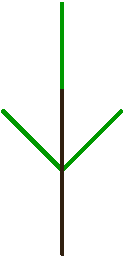
\includegraphics[scale=1]{Branching1}
		~
	} ~
	\subfloat[Second iteration]{
		\includegraphics[scale=1]{Branching2}
	} ~
	\subfloat[Third iteration]{
		\includegraphics[scale=1]{Branching3}
	} ~
	\subfloat[Fourth iteration]{
		\includegraphics[scale=1]{Branching4}
	}
	\caption{First four iterations of bracketed \lsystem \ref{lsys:branchingSrc}}
	\label{fig:branching}
\end{figure}



\subsection{Stochastic \lsystems}

\newcommand{\zerolsystem}{\mbox{0L-system}\xspace}
\newcommand{\zerolsystems}{\mbox{0L-systems}\xspace}

All plants generated by same deterministic \lsystem are identical.
Forest made by trees which are identical looks artificial and can not be used in films or video games.
Stochastic \lsystems solves this problem because they can produce randomized model.
Stochastic \lsystems are called \zerolsystem where 0 means they are context-free.

Randomization of model produced by \lsystem can be done in two places, in rewrite rules or in interpretation of symbols (or in both).
Randomization in interpretation can only change properties of interpreted symbols such as lengths of lines or turning angles, the topology of plant remains unchanged.
In contrast with rewrite rule randomization which can also change topology of model.
Rewrite rule randomization is done by defining more replacements for one rewrite rule.
Rewriting system will pick random replacement if rewrite rule is applied.
Each replacement can have different probability to be picked.

On figure \ref{fig:randComparison} are shown 3 models of plant generated by stochastic \lsystems.
First image \ref{fig:randComparisonNo} was generated without any randomization.
Second image \ref{fig:randComparisonInt} was generated with interpretation randomization of line lengths and angles.
For last image \ref{fig:randComparisonBoth} was also added topology randomization with rewrite rule randomization.
Source code for the last image is shown in figure \ref{lsys:randExample}.

\begin{figure}[ht]
	\centering
	\subfloat[No randomization]{
		\label{fig:randComparisonNo}
		\includegraphics[width=0.3\textwidth]{StochasticLsystemExample-NoStochasism}
	} ~
	\subfloat[Angles, lengths randomized]{
		\label{fig:randComparisonInt}
		\includegraphics[width=0.32\textwidth]{StochasticLsystemExample-InterpretationStochasism}
	} ~
	\subfloat[Also topology randomized]{
		~
		\label{fig:randComparisonBoth}
		\includegraphics[width=0.25\textwidth]{StochasticLsystemExample-BothStochasism}
		~
	}
	\caption{Comparison between non-randomized and randomized plant model}
	\label{fig:randComparison}
\end{figure}

\begin{Lsystem}[label=lsys:randExample,caption={Example of stochastic \lsystem with randomized rewrite rules and interpretation}]
lsystem StochasticLsystemExample {
	set symbols axiom = X;
	set initialAngle = 90;
	set iterations = 8;
	set randomSeed = 1036793868;

	interpret F(age) as DrawForward(1.8^age*random(0.5,1.5), age/2);
	interpret + as TurnLeft(45 + random(-20, 20));
	interpret - as TurnLeft(-45 + random(-20, 20));
	interpret [ as StartBranch;
	interpret ] as EndBranch;

	rewrite F(age) to F(age + 1);
	rewrite X
		to F(1) [ + X ] [ - X ] F(1) X  weight 4 or
		to F(1) [ + X ]         F(1) X  weight 1 or
		to F(1)         [ - X ] F(1) X  weight 1;
}
process all with SvgRenderer;
\end{Lsystem}


\subsection{Context-sensitive \lsystems}

\newcommand{\onelsystems}{\mbox{1L-systems}\xspace}
\newcommand{\twolsystems}{\mbox{2L-systems}\xspace}

Rewriting of symbols in \zerolsystems is context-free, rewrite rules are applied on the symbols regrades of their context (symbols around it).
However rewriting of symbol can also depend on its context.
This is useful in simulating the flow of signals (nutrients or hormones) in plant model~\citep{PL91}.

Formally there are two types of context sensitive L-systems, \onelsystems and \twolsystems.
Rewrite rules of \onelsystems checks context only on one side (left or right) whereas rewrite rules of \twolsystems checks context on both sides.
Since \onelsystems are just \twolsystems with one context empty we will consider context sensitive \lsystems as \twolsystems.

Context sensitive \lsystem \ref{lsys:signalPropagarionSrc} shows simulation of signal propagation in the string of symbols.
Result is in table \ref{fig:signalPropagarion}.

\begin{Lsystem}[label=lsys:signalPropagarionSrc,caption={Context-sensitive \lsystems simulating signal propagation}]
lsystem RewritingExample {
	set symbols axiom = B A A A A A;
	set iterations = 6;
	set interpretEveryIteration = true;
	rewrite {B} A     to B;
	rewrite     B {A} to A;
}
process all with SymbolPrinter;
\end{Lsystem}

\begin{table}[ht]
	\centering
	\begin{tabular}{c l}
   		\toprule
   		Iteration & String of symbols \\
   		\midrule
		0 & B A A A A A \\
		1 & A B A A A A \\
		2 & A A B A A A \\
		3 & A A A B A A \\
		4 & A A A A B A \\
		5 & A A A A A B \\
		6 & A A A A A A \\
		\bottomrule
	\end{tabular}
	\caption{Axiom and first 6 iterations of \lsystem \ref{lsys:signalPropagarionSrc} showing signal propagation in the string of symbols}
	\label{fig:signalPropagarion}
\end{table}


\subsubsection{Context-sensitive bracketed \lsystems}

If we add context-sensitive rewrite rule to bracketed \lsystems situation will be more difficult.
The context matching procedure must take into account branches.
Following rules defines natural behavior of context between branches:
\begin{enumerate*}
	\item \label{enum:ctxRule1} two symbols are neighbors even if there are some branches between them,
	\item \label{enum:ctxRule2} left neighbor of first symbol in branch is symbol before branch,
	\item \label{enum:ctxRule3} last symbol in branch do not have right neighbor,
	\item \label{enum:ctxRule4} unmatched symbols at the end of branch are ignored,
	\item \label{enum:ctxRule5} order of branches is insignificant.
\end{enumerate*}

Table \ref{tbl:bracketCtxt} shows examples of context matching in bracketed \lsystems with references to according rules.

\begin{table}[ht]
	\centering
	\begin{tabular}{c c c p{128pt} c c}
   		\toprule
   		Left ctx. & Symbol & Right ctx. & Symbol string & Match & Rule\\
   		\midrule
		 & X & Y & A B \textbf{X} [ A [ B ] ] [ C ] \textbf{Y} & yes & \ref{enum:ctxRule1} \\
		 & X & Y & A B \textbf{X} [ Y B ] C Y & no &  \\
		 Y & X & & A B \textbf{Y} [ \textbf{X} A B ] C & yes & \ref{enum:ctxRule2} \\
		 Y & X & & A B \textbf{Y} [ [ \textbf{X} A ] B ] C & yes & \ref{enum:ctxRule2} \\
		 & X & Y & A [ B \textbf{X} ] Y & no & \ref{enum:ctxRule3} \\
		 & X & [ Y ] & A B \textbf{X} [ \textbf{Y} A B ] A  & yes & \ref{enum:ctxRule4} \\
		 & X & [ [ Y ] ] & A B \textbf{X} [ [ \textbf{Y} A B ] C ] & yes & \ref{enum:ctxRule4} \\
		 & X & [ Y ] & A B \textbf{X} [ A B ] [ \textbf{Y} ] A  & yes & \ref{enum:ctxRule5} \\
		 & X & [ Y ] [ Z ] & A B \textbf{X} [ \textbf{Z} ] [ \textbf{Y} ] A  & yes & \ref{enum:ctxRule5} \\
		\bottomrule
	\end{tabular}
	\caption{Examples of context matching in bracketed \lsystems}
	\label{tbl:bracketCtxt}
\end{table}

Context in bracketed \lsystems can be used for propagation of signals through tree structure.
There are two basic types of signals.
First is \emph{acropetal} signal which spreads from root to branches and second is \emph{basipetal} which spreads in other way i.e. from branches to root.
This can be used well in plant modeling.

Figure \ref{fig:signalPropagation} shows simulation of acropetal (\ref{fig:acropetalSignal}) and basipetal (\ref{fig:basipetalSignal}) signals in static plant-like structure.
Each figure shows first 5 iterations and segments with signal are marked bolder.

\begin{figure}[ht]
	\centering
	\subfloat[Acropetal signal propagation]{
		\includegraphics[scale=0.5]{AcropetalSignal1}\hspace{1mm}
		\includegraphics[scale=0.5]{AcropetalSignal2}\hspace{1mm}
		
\includegraphics[scale=0.5]{AcropetalSignal3}\hspace{1mm}
		\includegraphics[scale=0.5]{AcropetalSignal4}\hspace{1mm}
		\includegraphics[scale=0.5]{AcropetalSignal5}
		\label{fig:acropetalSignal}
	}
	\hfill
	\subfloat[Basipetal signal propagation]{
		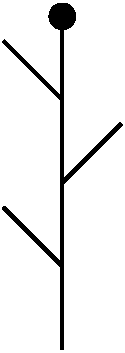
\includegraphics[scale=0.5]{BasipetalSignal1}\hspace{2mm}
		\includegraphics[scale=0.5]{BasipetalSignal2}\hspace{2mm}
		\includegraphics[scale=0.5]{BasipetalSignal3}\hspace{2mm}
		\includegraphics[scale=0.5]{BasipetalSignal4}\hspace{2mm}
		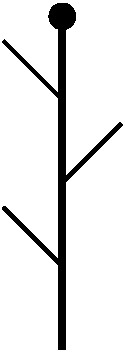
\includegraphics[scale=0.5]{BasipetalSignal5}
		\label{fig:basipetalSignal}
	}
	\caption{Signal propagation simulated with context-sensitive bracketed \lsystems}
	\label{fig:signalPropagation}
\end{figure}


\subsection{Parametric \lsystems}

Symbols in parametric \lsystems can hold any number of arguments.
Arguments are often floating point numbers but they can be more complicated structures.
Arguments can be used in interpretation definition to send values like length of line or color to interpretation routine.
Arguments can be also used in rewrite rules to determine whether rewrite symbol or not and to determine new arguments for rewritten symbols.
In context \twolsystems is also possible to get arguments from symbols in context and use them in rewrite rules.






































\clearpage

\section{\lsystem types}
\label{sec:lsysTypes}

In this section is described different types of \lsystems.
Some types may require an extension to the described formal definition of an \lsystem but this will be omitted here.

The \lsystems described so far are called \emph{deterministic \lsystems} because their rewriting system is deterministic.
\emph{Bracketed \lsystems} allow to save and load a state of the interpretation;
	this can be used to model branches of plants more easily.
\emph{Stochastic \lsystems} can randomize a result model to suppress its artificiality.
\emph{Context-sensitive \lsystems} allow to rewrite symbols depending on their context (the neighboring symbols around them).
Symbols in \emph{parametric \lsystems} can hold any number of arguments that can be used while rewriting or interpreting symbols.

Any of the above-described types can be combined together.



\subsection{Deterministic \lsystems}

\newcommand{\dzerolsystem}{\mbox{D0L-system}\xspace}
\newcommand{\dlsystem}{\mbox{dL-system}\xspace}


\begin{wrapfigure}{r}{0.50\textwidth}
	\vspace{-30pt}
	\includegraphics[width=\linewidth]{BasicLsystem}
	\caption{Dragon curve}
	\label{fig:basicLsystem}
\end{wrapfigure}


The basic \lsystem type described by the previous formal definition is called a \dzerolsystem\footnote{A \dzerolsystem is also just called a \dlsystem~\cite{Zar04}.}.
\emph{D} means that the rewriting is deterministic and \emph{0} means it is context-free.
The result of a \dzerolsystem depends only on the initial string of symbols.

This type of \lsystem is often used to generate fractal curves.
With the \dzerolsystem in \autoref{fig:basicLsystem} we can generate the Dragon curve that you can see in \autoref{lsys:basicLsystemSrc}.

\begin{Lsystem}[label=lsys:basicLsystemSrc,caption={\dzerolsystem for the generation of the Dragon curve (\autoref{fig:basicLsystem})}]
lsystem DragonCurve {
	set iterations = 12;
	set symbols axiom = L;
	interpret R L as DrawForward(5);
	interpret + as TurnLeft(90);
	interpret - as TurnLeft(-90);
	rewrite L to L + R +;
	rewrite R to - L - R;
}
process all with SvgRenderer;
\end{Lsystem}


\subsection{Bracketed \lsystems}

A bracketed \lsystems\cite[p.~24]{PL91} extends basic \dzerolsystem with a branching system.
Branching is such a fundamental feature that Bracketed \lsystems are often just called \lsystems.

A branching system brings two new commands to the symbol interpretation system: \emph{start branch} and \emph{end branch}.
These commands are nearly always represented as bracket symbols (from which bracketed \lsystems got their name).
An open bracket "\texttt{[}" as a start branch and close bracket "\texttt{]}" as a close branch.

The start branch command saves the state of interpretation, which can then be loaded by end the branch command later.
In turtle graphics, the interpretation state is the position, orientation and drawing color of the turtle.
More than one state can be saved at the same time, and the last saved state will be loaded first.
This behavior seems natural and could be compared to a pairing of brackets.

Branching extends a linear string of symbols to a tree structure.
Individual branches do not affect each other nor their root.
This allows plants to be modeled more easily and to create more complex models.

The bracketed \lsystem in \autoref{lsys:branchingSrc} demonstrates a use of the branching system to produce a plant-like model as can be seen in \autoref{fig:branching}.
Note that the color of segments indicates their type and age.
Black segments are drawn with the symbol \texttt{F} and they represent segments from the previous iteration.
Green segments are drawn with the symbol \texttt{A} and they are new compared to the previous iteration.

\begin{Lsystem}[label=lsys:branchingSrc,caption={A bracketed \lsystem that which creates a plant-like model (\autoref{fig:branching})}]
lsystem PythagorasTree {
	set symbols axiom = A;
	set initialAngle = 90;
	set iterations = 4;	
	interpret A F as DrawForward(16);
	interpret + as TurnLeft(45);
	interpret - as TurnLeft(-45);
	@interpret [ as StartBranch;@
	@interpret ] as EndBranch;@
	rewrite A to F [ + A ] [ - A ] F A;
	rewrite F to F F;
}
process all with SvgRenderer;
\end{Lsystem}

\begin{figure}[h]
	\centering
	\subfloat{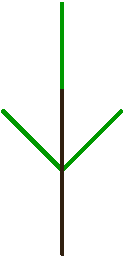
\includegraphics[scale=1]{Branching1}} ~
	\subfloat{\includegraphics[scale=1]{Branching2}} ~
	\subfloat{\includegraphics[scale=1]{Branching3}} ~
	\subfloat{\includegraphics[scale=1]{Branching4}}
	\caption[The first four iterations of a bracketed \lsystem]{The first four iterations of the bracketed \lsystem in \autoref{lsys:branchingSrc}}
	\label{fig:branching}
\end{figure}



\subsection{Stochastic \lsystems}

\newcommand{\zerolsystem}{\mbox{0L-system}\xspace}
\newcommand{\zerolsystems}{\mbox{0L-systems}\xspace}

All plant models generated by the same deterministic \lsystem are identical.
However, a forest made by trees which are all identical looks artificial and can not be used in films or video games.
Stochastic \lsystems solve this problem because they can produce a randomized model.
Stochastic \lsystems are called \zerolsystem where 0 means they are context-free.

Randomization of a model produced by stochastic a \lsystem can be done in two places, in the rewrite rules or in the interpretation of symbols (or in both).
Randomization in interpretation can only change the properties of such interpreted symbols as lengths of lines or turning angles, while the topology of the model remains unchanged.
This is in contrast to rewrite rule randomization that can also change the topology of a model.
Rewrite rule randomization is achieved by defining more replacements for one rewrite rule.
The rewriting system will pick a random replacement if the rewrite rule is applied.
Each replacement can have a different probability of being picked.

In \autoref{fig:randComparison}, three models of a plant generated by stochastic \lsystems are shown.
The first image (\ref{fig:randComparisonNo}) was generated without any randomization.
The second image (\ref{fig:randComparisonInt}) was generated with interpretation randomization of line lengths and angles.
For the last image (\ref{fig:randComparisonBoth}) was used the rewrite rule randomization which changed the topology of the model (\autoref{lsys:randExample}).

\begin{figure}[h]
	\centering
	\subfloat[No randomization]{
		\label{fig:randComparisonNo}
		\includegraphics[width=0.3\textwidth]{StochasticLsystemExample-NoStochasism}
	} ~
	\subfloat[Angles, lengths randomized]{
		\label{fig:randComparisonInt}
		\includegraphics[width=0.32\textwidth]{StochasticLsystemExample-InterpretationStochasism}
	} ~
	\subfloat[Also topology randomized]{
		~
		\label{fig:randComparisonBoth}
		\includegraphics[width=0.25\textwidth]{StochasticLsystemExample-BothStochasism}
		~
	}
	\caption{A comparison between a non-randomized and randomized plant model}
	\label{fig:randComparison}
\end{figure}

\begin{Lsystem}[label=lsys:randExample,caption={Stochastic \lsystem with randomized interpretation of symbols and rewrite rule replacements}]
lsystem StochasticLsystemExample {
	set symbols axiom = X;
	set iterations = 8;
	set initialAngle = 90;
	interpret F(age) as DrawForward(@1.8^age*random(0.5,1.5)@, age/2);
	interpret + as TurnLeft(@45 + random(-20, 20)@);
	interpret - as TurnLeft(@-45 + random(-20, 20)@);
	interpret [ as StartBranch;
	interpret ] as EndBranch;
	rewrite F(age) to F(age + 1);
	@rewrite X@
		@to F(1) [ + X ] [ - X ] F(1) X  weight 4 or@
		@to F(1) [ + X ]         F(1) X  weight 1 or@
		@to F(1)         [ - X ] F(1) X  weight 1;@
}
process all with SvgRenderer;
\end{Lsystem}


\subsection{Context-sensitive \lsystems}

\newcommand{\onelsystems}{\mbox{1L-systems}\xspace}
\newcommand{\twolsystems}{\mbox{2L-systems}\xspace}

The rewriting of symbols in \zerolsystems is context-free; the rewrite rules are applied to the symbols regardless of their context (the symbols around them).
However, the rewriting of a symbol can also depend on its context.
This is useful in simulating the flow of signals (nutrients or hormones) in a plant model that, for example, attempts to demonstrate natural plant growth~\citep{PL91}.

Formally there are two types of context-sensitive L-systems, \onelsystems and \twolsystems.
The rewrite rules of \onelsystems checks the context only to one side (left or right), whereas the rewrite rules of \twolsystems checks the context on both sides.
Since \onelsystems are just \twolsystems with one context empty we will consider context-sensitive \lsystems as \twolsystems.

The context-sensitive \lsystem in \autoref{lsys:signalPropagarionSrc} shows a simulation of signal propagation in a string of symbols; the result is given in \autoref{fig:signalPropagarion}.

\begin{Lsystem}[label=lsys:signalPropagarionSrc,caption={Context-sensitive \lsystem simulating signal propagation}]
lsystem RewritingExample {
	set symbols axiom = B A A A A A;
	set iterations = 6;
	set interpretEveryIteration = true;
	@rewrite {B} A     to B;@
	@rewrite     B {A} to A;@
}
process all with SymbolPrinter;
\end{Lsystem}

\begin{table}[h]
	\centering
	\begin{tabular}{c l}
   		\toprule
   		Iteration & String of symbols \\
   		\midrule
		0 & B A A A A A \\
		1 & A B A A A A \\
		2 & A A B A A A \\
		3 & A A A B A A \\
		4 & A A A A B A \\
		5 & A A A A A B \\
		6 & A A A A A A \\
		\bottomrule
	\end{tabular}
	\caption{An axiom and the first 6 iterations of an \lsystem in \autoref{lsys:signalPropagarionSrc} showing signal propagation in the given string of symbols}
	\label{fig:signalPropagarion}
\end{table}


\subsubsection{Context-sensitive bracketed \lsystems}
\label{sec:bracketedLsystems}

If we add context-sensitive rewrite rules to bracketed \lsystems the situation becomes more difficult.
The context-matching procedure must take into account the branches.
The following rules define the natural behavior of context between branches:
\begin{enumerate*}
	\item \label{enum:ctxRule1} two symbols are neighbors even if there are some branches between them,
	\item \label{enum:ctxRule2} the left neighbor of the first symbol in a branch is a symbol before the branch,
	\item \label{enum:ctxRule3} the last symbol in a branch does not have a right neighbor,
	\item \label{enum:ctxRule4} unmatched symbols at the end of a branch are ignored,
	\item \label{enum:ctxRule5} the order of branches is insignificant.
\end{enumerate*}

In \autoref{tbl:bracketCtxt} is a few examples of how a symbol with its context will match (or not) a given string of symbols with respect to the context-matching rules mentioned above.
\begin{table}[h]
	\centering
	\begin{tabular}{c c c | p{128pt} c c}
   		\toprule
   		Left ctx. & Symbol & Right ctx. & Symbol string & Match & Rule\\
   		\midrule
		 & X & Y & A B {\btHL\bf X} [ A [ B ] ] [ C ] {\btHL\bf Y} & yes & \ref{enum:ctxRule1} \\
		 & X & Y & A B X [ Y B ] C Y & no &  \\
		 Y & X & & A B {\btHL\bf Y [ X} A B ] C & yes & \ref{enum:ctxRule2} \\
		 Y & X & & A B {\btHL\bf Y [ [ X} A ] B ] C & yes & \ref{enum:ctxRule2} \\
		 & X & Y & A [ B X ] Y & no & \ref{enum:ctxRule3} \\
		 & X & [ Y ] & A B {\btHL\bf X [ Y} A B ] A  & yes & \ref{enum:ctxRule4} \\
		 & X & [ [ Y ] ] & A B {\btHL\bf X [ [ Y} A B ] C ] & yes & \ref{enum:ctxRule4} \\
		 & X & [ Y ] & A B {\btHL\bf X} [ A B ] {\btHL\bf{}[ Y} ] A  & yes & \ref{enum:ctxRule5} \\
		 & X & [ Y ] [ Z ] & A B {\btHL\bf X [ Z} ] {\btHL\bf{}[ Y} ] A  & yes & \ref{enum:ctxRule5} \\
		\bottomrule
	\end{tabular}
	\caption{Examples of context matching in bracketed \lsystems}
	\label{tbl:bracketCtxt}
\end{table}

Context in bracketed \lsystems can be used for the propagation of signals through tree structures.
There are two basic types of signals: the first is the \emph{acropetal} signal which spreads from the root to branches; and the second signal is \emph{basipetal} which spreads in the opposite way i.e. from branches to root.
This can be very useful in plant modeling.

\autoref{fig:signalPropagation} shows a simulation of acropetal (\ref{fig:acropetalSignal}) and basipetal (\ref{fig:basipetalSignal}) signals in a static plant-like structure.
Each figure shows the first 5 iterations and segments with the signal marked as a bolder line.
The \lsystem in \autoref{lsys:signalPropagation} simulates acropetal signal propagation and its result is in \autoref{fig:acropetalSignal} (image) and \autoref{fig:signalPropagationTable} (symbols).

\begin{figure}[h!]
	\centering
	\subfloat[Acropetal signal propagation]{
		\includegraphics[scale=0.55]{AcropetalSignal}
		\label{fig:acropetalSignal}
	}
	\hspace{2mm}
	\subfloat[Basipetal signal propagation]{
		\includegraphics[scale=0.55]{BasipetalSignal}
		\label{fig:basipetalSignal}
	}
	\caption{Signal propagation simulated with context-sensitive bracketed \lsystems}
	\label{fig:signalPropagation}
\end{figure}

\begin{Lsystem}[label=lsys:signalPropagation,caption={The \lsystem simulating acropetal signal propagation (\autoref{fig:acropetalSignal})}]
lsystem AcropetalSignal extends Branches {
	set symbols axiom = B [ + A ] A [ - A ] A [ + A ] A;
	// ignore + and - symbols in context search
	@set symbols contextIgnore = + -;@
	set iterations = 3;
	// interpret every iteration to see signal propagation
	set interpretEveryIteration = true;
	set initialAngle = 90;
	interpret A as DrawForward(50, 2);
	interpret B as DrawForward(50, 4);
	interpret + as TurnLeft(45);
	interpret - as TurnLeft(-45);
	@rewrite { B } A to B;@
}
process all with SvgRenderer;
\end{Lsystem}


\begin{table}[h]
	\centering
	\begin{tabular}{c c}
   		\toprule
   		Iteration & String of symbols \\
   		\midrule
		0 & B [ + A ] A [ - A ] A [ + A ] A \\
		1 & B [ + B ] B [ - A ] A [ + A ] A \\
		2 & B [ + B ] B [ - B ] B [ + A ] A \\
		3 & B [ + B ] B [ - B ] B [ + B ] B \\
		\bottomrule
	\end{tabular}
	\caption{The result of the \lsystem simulating acropetal signal propagation in \autoref{lsys:signalPropagation}}
	\label{fig:signalPropagationTable}
\end{table}


\subsection{Parametric \lsystems}

Symbols in parametric \lsystems can hold any number of arguments.
Arguments are often floating point numbers, but they can be much more complicated structures.
Arguments can be used in interpretation definition to send values like color or length of line to an interpretation routine.
Arguments can also be used in rewrite rules to determine whether to rewrite a symbol or not, and to determine new arguments for rewritten symbols.
In context \twolsystems it is also possible to get arguments from symbols in context and use them in rewrite rules.

The \lsystem in \autoref{fig:scParams} shows an example of how the parameters of symbols can be used in interpretation methods and in rewrite rules together with the result.

\newsavebox{\lstBox}
\begin{lrbox}{\lstBox}
\begin{Lsystem50}
lsystem Circles {
	set symbols axiom =	[ X ] +
		[ X ] + [ X ] + [ X ];
	set iterations = 7;
	interpret F as MoveForward;
	interpret K as DrawCircle;
	interpret + as @TurnLeft(90)@;
	interpret - as @TurnLeft(-90)@;
	interpret [ as StartBranch;
	interpret ] as EndBranch;
	rewrite @K(n) to K(2*n)@;
	rewrite @F(n) to F(2*n)@;
	rewrite X to @K(2) F(3)@
		[ + X ] [ - X ] X;
}
process all with SvgRenderer;
\end{Lsystem50}
\end{lrbox}

\begin{figure}[h!]
	\subfloat{
		\usebox{\lstBox}
	} \hfill
	\subfloat{
		\minipage{0.47\linewidth}\noindent
		\includegraphics[width=\textwidth]{Circles}
		\endminipage
	}
	\caption{Parameters usage in \lsystem interpretation methods and in rewrite rules along with the result}
	\label{fig:scParams}
\end{figure}

In \autoref{fig:redEndPythagoras} is more complicated model, the Pythagoras tree.
Detailed instructions for its construction with \lsystems are described in appendix \ref{chap:userDoc}.

\begin{figure}[H]
	\centering
	\includegraphics[width=\linewidth]{PythagorasTree2dRedEnd}
	\caption{Pythagoras tree created with parametric \lsystem}
	\label{fig:redEndPythagoras}
\end{figure}


































\clearpage

\section{Related \lsystem generators}

In this section will be listed other computer programs or web pages that allows to process \lsystems and eventually interpret them in most cases as an image.

\subsection{Web based}
\label{sec:WebBasedGenerators}

\subsubsection{\lsystem generator by Michael Norris}
{ \vspace{-10pt} \footnotesize \url{http://www.michaelnorris.info/software/l-system-generator.html} }

Simple script which offers to set basic properties of L-system namely number of iterations, axiom and up to 15 rewrite rules.
Result is list of strings of symbols from all iterations (it does not interpret symbols).


\subsubsection{Lindenmayer power by MadFlame Software}
{ \vspace{-10pt} \footnotesize \url{http://madflame991.blogspot.com/p/lindenmayer-power.html} }

L-system generator which offers to set basic properties of L-system and interpretation for each symbol.
Symbols can be interpreted as turtle graphics or they can define or modify value of variable.
All iterations are listed as text and drawn on screen as well.


\subsubsection{\lsystem generator by Nolan Carroll}	
{ \vspace{-10pt} \footnotesize \url{http://nolandc.com/sandbox/fractals/} }

L-system generator with quite nice interface where is possible to set basic properties of L-system and interpretation.
Interpretation of symbols is unchangeable.
Last iteration of L-system is drawn on screen.


\subsubsection{VRML \lsystem generator by Patrick Murris}
{ \vspace{-10pt} \footnotesize \url{http://www.alpix.com/vrml/lsys.htm} }
  
L-system generator which can generate 3D VRML model.
Basic properties of L-system and interpretation can be set.
Only problem is that VRML plugin is needed for displaying 3D models.


\subsubsection{\lsystem generator by John Snyders}
{ \vspace{-10pt} \footnotesize \url{http://hardlikesoftware.com/projects/lsystem/lsystem.html} }
  
At first sight quite sophisticated L-system generator which can rewrite symbols with parameters and do context-sensitive rewriting.
Result is drawn on page as animation of development.
Biggest drawback is that L-systems are hard-coded in JavaScript and it is only possible to browse them in different iterations.



\subsection{Desktop applications}
\label{sec:DesktopGenerators}

\subsubsection{L-studio by Przemysław Prusinkiewicz et. al}
{ \vspace{-10pt} \footnotesize \url{http://algorithmicbotany.org/lstudio/} }

\begin{wrapfigure}{r}{0.5\textwidth}
	\vspace{-20pt}
	\begin{center}
	\includegraphics[width=0.48\textwidth]{Lily}
	\end{center}
	\caption{Model of Lily produced by L-studio}
\end{wrapfigure}

L-studio is one of the best applications for modeling plants with \lsystems (it is also possible to create general fractals with it).
L-studio is not single program but it is complex solution that consists of many tools.
With L-studio it is possible to model 3D models of plants with regards to environment like wind, gravity, space the around plant, sun light, etc.
Output can be saved in many formats like Wavefront OBJ, Postscript, BMP or render plant with built in ray-tracer to produce photo-realistic images.

Even there is many examples of plant models and extensive help it is not easy to start using it.
The syntax is very compact and quite unclear.

Application is not free-ware but demo version can be downloaded.
After evaluation period it is still possible to use it but it is not possible to export images and previews have watermark. 


\subsubsection{\lsystems explorer by James Matthews}
{ \vspace{-10pt} \footnotesize \url{http://www.generation5.org/content/2002/lse.asp} }
\label{sec:LsystemExplorer}

Simple desktop application which renders L-systems in window.
Basic properties of \lsystem and its interpretation can be edited in dialog window but interpretation for individual symbols can not be changed.
\lsystems can be saved or loaded into text file but drawn image can not be saved.


\subsubsection{\lsystem Vector Generator by Dmitry Malutin}
{ \vspace{-10pt} \footnotesize \url{http://xaraxtv.at.tut.by/lsvg.htm} }

Similar application to \nameref{sec:LsystemExplorer} but it is also possible to randomize line lengths or turn angles.
Nice feature is \emph{angle wizard} which displays grid \lsystems each with different setting of turn angle.
It is possible to save image as AI or WMF which are not most common formats.


\subsubsection{L-System 4 by Timothy Perz}
{ \vspace{-10pt} \footnotesize \url{http://www.oocities.org/tperz/L4About.htm} }

L-System 4 is quite advanced tool for generating models with \lsystems.
Besides all basic functionality it is possible to create 3D models with textures.
Models can be saved to raster images as BMP or JPEG or they can be exported to AutoCAD DXF format.
Interpreting capabilities are quite good but \lsystem rewriting can do only deterministic rewriting with limited usage of parameters.


























































%
\section{Related \lsystem generators}

In this section will be listed other computer programs or web pages that allows to process \lsystems and eventually interpret them in most cases as an image.

\subsection{Web based}
\label{sec:WebBasedGenerators}

\subsubsection{\lsystem generator by Michael Norris}
{ \vspace{-10pt} \footnotesize \url{http://www.michaelnorris.info/software/l-system-generator.html} }

Simple script which offers to set basic properties of L-system namely number of iterations, axiom and up to 15 rewrite rules.
Result is list of strings of symbols from all iterations (it does not interpret symbols).


\subsubsection{Lindenmayer power by MadFlame Software}
{ \vspace{-10pt} \footnotesize \url{http://madflame991.blogspot.com/p/lindenmayer-power.html} }

L-system generator which offers to set basic properties of L-system and interpretation for each symbol.
Symbols can be interpreted as turtle graphics or they can define or modify value of variable.
All iterations are listed as text and drawn on screen as well.


\subsubsection{\lsystem generator by Nolan Carroll}	
{ \vspace{-10pt} \footnotesize \url{http://nolandc.com/sandbox/fractals/} }

L-system generator with quite nice interface where is possible to set basic properties of L-system and interpretation.
Interpretation of symbols is unchangeable.
Last iteration of L-system is drawn on screen.


\subsubsection{VRML \lsystem generator by Patrick Murris}
{ \vspace{-10pt} \footnotesize \url{http://www.alpix.com/vrml/lsys.htm} }
  
L-system generator which can generate 3D VRML model.
Basic properties of L-system and interpretation can be set.
Only problem is that VRML plugin is needed for displaying 3D models.


\subsubsection{\lsystem generator by John Snyders}
{ \vspace{-10pt} \footnotesize \url{http://hardlikesoftware.com/projects/lsystem/lsystem.html} }
  
At first sight quite sophisticated L-system generator which can rewrite symbols with parameters and do context-sensitive rewriting.
Result is drawn on page as animation of development.
Biggest drawback is that L-systems are hard-coded in JavaScript and it is only possible to browse them in different iterations.



\subsection{Desktop applications}
\label{sec:DesktopGenerators}

\subsubsection{L-studio by Przemysław Prusinkiewicz et. al}
{ \vspace{-10pt} \footnotesize \url{http://algorithmicbotany.org/lstudio/} }

\begin{wrapfigure}{r}{0.5\textwidth}
	\vspace{-20pt}
	\begin{center}
	\includegraphics[width=0.48\textwidth]{Lily}
	\end{center}
	\caption{Model of Lily produced by L-studio}
\end{wrapfigure}

L-studio is one of the best applications for modeling plants with \lsystems (it is also possible to create general fractals with it).
L-studio is not single program but it is complex solution that consists of many tools.
With L-studio it is possible to model 3D models of plants with regards to environment like wind, gravity, space the around plant, sun light, etc.
Output can be saved in many formats like Wavefront OBJ, Postscript, BMP or render plant with built in ray-tracer to produce photo-realistic images.

Even there is many examples of plant models and extensive help it is not easy to start using it.
The syntax is very compact and quite unclear.

Application is not free-ware but demo version can be downloaded.
After evaluation period it is still possible to use it but it is not possible to export images and previews have watermark. 


\subsubsection{\lsystems explorer by James Matthews}
{ \vspace{-10pt} \footnotesize \url{http://www.generation5.org/content/2002/lse.asp} }
\label{sec:LsystemExplorer}

Simple desktop application which renders L-systems in window.
Basic properties of \lsystem and its interpretation can be edited in dialog window but interpretation for individual symbols can not be changed.
\lsystems can be saved or loaded into text file but drawn image can not be saved.


\subsubsection{\lsystem Vector Generator by Dmitry Malutin}
{ \vspace{-10pt} \footnotesize \url{http://xaraxtv.at.tut.by/lsvg.htm} }

Similar application to \nameref{sec:LsystemExplorer} but it is also possible to randomize line lengths or turn angles.
Nice feature is \emph{angle wizard} which displays grid \lsystems each with different setting of turn angle.
It is possible to save image as AI or WMF which are not most common formats.


\subsubsection{L-System 4 by Timothy Perz}
{ \vspace{-10pt} \footnotesize \url{http://www.oocities.org/tperz/L4About.htm} }

L-System 4 is quite advanced tool for generating models with \lsystems.
Besides all basic functionality it is possible to create 3D models with textures.
Models can be saved to raster images as BMP or JPEG or they can be exported to AutoCAD DXF format.
Interpreting capabilities are quite good but \lsystem rewriting can do only deterministic rewriting with limited usage of parameters.

























\chapter{Design}

In this chapter the design of my solution for an online feature-rich development environment is described and the decisions that were made explained.
Implementation details are described in \autoref{chap:implementation}.

In the first section (\ref{sec:design-library}) the design of the \lsystem processing library is described.
The library processes input with a component-based approach.
The core of the library is responsible for creating system a of connected components (components graph) but processing of the \lsystem itself is fully under the control of the components.
Components can be created by the user, thus bringing freedom to the \lsystem processing.

The library contains predefined components to make it possible to process \lsystems without need the for creating custom components.
The design of these components is described in the second section (\ref{sec:design-components}).
Predefined components also serves as an example for users who want to implement their own components or whole processing system.

In the third section (\ref{sec:design-web}) is described the design of the online web user interface.
It uses the library and components to process input so it also serves as an example of the usage of the library.


\section{Choice of development environment}

As development environment was chosen the .NET framework because of following reasons.

\begin{description*}
	\item[Multiplatformity]
		Thanks to the Mono project\footnote{Mono is an open source implementation of Microsoft's .NET Framework (\url{http://www.mono-project.com}).}
			.NET libraries and executables can be used not only on Windows but also on Linux, Mac and many other operating systems.
	\item[Development tools]
		Visual Studio 2010 is powerful integrated development environment (IDE) with many integrated tools (like inteli-sense, NuGet package system or T4 templates) and useful downloadable plugins.
		Visual Studio has built-in support for unit testing which helps to test especially non-runnable code like libraries easily.
		\nomenclature{IDE}{integrated development environment}
		\nomenclature{T4}{text template transformation toolkit}
	\item[Reflection]
		Reflection is the ability to examine types and work with meta-data, properties and functions of an object at runtime.
		Reflection can be used to load various plugins or data at runtime and help extensibility in great way.
	\item[Parser generator]
		FsLex and FsYacc are lexer and parser generators written in F\# with good support by Visual Studio.
		Generated lexer and parser are also in F\# thus they can be easily used in any .NET project.
	\item[Web framework]
		ASP.NET MVC is a lightweight presentation framework for creating web applications in .NET.
		ASP.NET MVC 3 is using the Razor view engine which helps to do the web very easily.
		\nomenclature{MVC}{model-view-controller (design pattern)}
	\item[Database and object mapping]
		MsSQL server offers to create database stored as a file directly in the application folder.
		Access to the database can be done using ADO.NET Entity Framework (EF) which can do an object-relational mapping (ORM) of the database.
		\nomenclature{MsSQL}{Microsoft SQL (server)}
		\nomenclature{SQL}{structured query language}
		\nomenclature{EF}{Entity framework}
		\nomenclature{ORM}{object-relational mapping}
\end{description*}



\section{\lsystem processing library design}

\lsystem processing library design will provide application interface (API) for processing of \lsystems.
The main feature will be extensibility....





















%\clearpage

\section{Processing system}
\label{sec:design-components}

As discussed in the previous chapter, the processing system of the library relies on the components.
The core of the library is responsible for just creating the component graph.
The processing of an \lsystem and production of results is fully under the control of the component graph.
This gives absolute freedom to the user in implementing the process system.

However it is hard to design and implement the whole \lsystem processing system from scratch.
The library contains a rich set of predefined components from which can be assembled many different component graphs.
The predefined components have a general interface which allows the user to reuse or extend them in order to add new functionality with a minimum of effort.


\subsection{Basic component system}

The component system designed in this section is primarily used for processing \lsystems to produce 2D and 3D graphics in the web interface.
However, the component system is designed to be extensible to any output type.

\lsystems are generally processed in two phases.
The first phase is rewriting where the axiom (the initial string of symbols) is rewritten by the rewrite rules, and the second phase is interpreting the resulting string of symbols.
This can be done with two components, the Rewriter -- which is responsible for rewriting the \lsystem to a given iteration -- and the Interpreter -- which is responsible for interpreting symbols and producing output (Fig. \ref{fig:simpleSystem}).

\begin{figure}[h!]
	\centering
	\begin{tikzpicture}[->,auto,node distance=3cm,>=latex,shorten >=2pt]
		\node (in) [coord] {};
		\node (rw) [block, right of=in] {Rewriter};
		\node (int) [block, right=1cm of rw] {Interpreter};
		\node (out) [coord, right of=int] {};
		
		\draw (in) -- node {input} (rw);
		\draw (rw) -- (int);
		\draw (int) -- node {output} (out);
	\end{tikzpicture}
	\caption{Simple \lsystem processing system}
	\label{fig:simpleSystem}
\end{figure}

However the components in the system in \autoref{fig:simpleSystem} have too many tasks to do, and thus they will be complicated to implement and hard to extend and test.

The system in \autoref{fig:advancedSystem} was created by a subdivision of the previous system.
The Rewriter component was split to the Rewriter and the Iterator.
The (new) Rewriter will just do the rewriting of some given symbols and the Iterator will control the iterating of the \lsystem (repetitive rewriting).
The Interpreter component was split to the Interpreter and the Renderer.
The (new) Interpreter will handle the interpreting of symbols: which means keep position of the virtual "turtle" in space, saving and loading of states, etc.
The Renderer will just produce the output.
If we need to create a different output type we only have to implement the new renderer component and the rest of the system will remain unchanged.

\begin{figure}[h!]
	\centering
	\begin{tikzpicture}[->,auto,node distance=3cm,>=latex,shorten >=2pt]
		\node (rw) [block] {Rewriter};
		\node (iter) [block, right of=rw] {Iterator};
		\node (in) [coord, above of=iter, node distance=15mm] {};
		\node (inter) [block, right of=iter] {Interpreter};
		\node (rend) [block, right of=inter] {Renderer};
		\node (out) [coord, right of=rend] {};
		
		\draw (rw) to[bend left=40] (iter);
		\draw (iter) to[bend left=40] (rw);
		\draw (in) -- node {input} (iter);
		\draw (iter) -- (inter);
		\draw (inter) -- (rend);
		\draw (rend) -- node {output} (out);
	\end{tikzpicture}
	\caption{Subdivided \lsystem processing system}
	\label{fig:advancedSystem}
\end{figure}


\subsection{Component system extensions}
\label{sec:caller}

The system in \autoref{fig:callerComponent} can be enhanced even more.
Every component that interprets \lsystem symbols needs to translate symbols to interpretation methods.
The translation can be implemented by every component individually.
However, the translation can be done by a specialized component called the \emph{Interpreter caller}.
This component can be smart enough to explore all the components in the system, find all the interpretation methods of all components and do translation automatically.
This causes an automatic "connection" of all interpreters to the interpreter caller.

More interpreters can be used to advantage: for example, for processing \lsystems which interact with themselves or their Environment \cite{MP96}.
One interpreter actually creates the result model and the second interpreter simulates the environment.

\begin{figure}[h!]
	\centering
	\begin{tikzpicture}[->,auto,node distance=3cm,>=latex,shorten >=2pt]
		\node (iter) [block] {Iterator};
		\node (in) [coord, above of=iter, node distance=15mm] {};
		\node (rw) [block, below of=iter, node distance=20mm] {Rewriter};
		\node (caller) [blockx, right of=iter, node distance=35mm] {Interpreter caller};
		\node (inter) [block, right of=caller, node distance=40mm] {Interpreter};
		\node (env) [block, below of=inter, node distance=20mm] {Environment module};
		\node (rend) [block, right of=inter] {Renderer};
		\node (out) [coord, right of=rend] {};
		
		\draw (rw) to[bend left=40] (iter);
		\draw (iter) to[bend left=40] (rw);
		\draw (in) -- node {input} (iter);
		\draw (iter) -- (caller);
		\draw [dashed] (caller) -- (inter);
		\draw [dashed] (caller) -- (env);
		\draw (inter) -- (rend);
		\draw (env) -- (rw);
		\draw (rend) -- node {output} (out);
	\end{tikzpicture}
	\caption[Automated interpreter caller]{The Interpreter caller which automatically calls interpretation methods of any components}
	\label{fig:callerComponent}
\end{figure}




The next necessary component is called the \emph{Random provider}.
It provides controlled behavior for random number generation as described in \autoref{sec:measuring}.
This component provides a function which returns a random number and it can be called by other components or by the user in the \lsystem definition.
This component is connected to the iterator to correctly the reset random seed at every pass.

The \emph{axiom provider} is the next extending component and it provides the axiom to the Iterator.
The axiom provider is only a "wrapper" around a single symbol property called the axiom.
The Iterator is designed generally to take the axiom from any component implementing \emph{ISymbolProvider} interface so it is possible to connect, for example, another rewriter as the axiom provider (Fig. \ref{fig:inputProvider}).

\begin{figure}[h!]
	\centering
	\begin{tikzpicture}[->,auto,node distance=3cm,>=latex,shorten >=2pt]
		\node (iter) [block] {Iterator};
		\node (rw) [block, left of=iter] {Main rewriter};
		\node (rw2) [blockx, above of=iter, node distance=20mm] {Input rewriter};
		\node (in) [coord, above of=rw2, node distance=15mm] {};
		\node (caller) [block, right of=iter, node distance=35mm] {Interpreter caller};
		\node (inter) [block, above of=caller, node distance=20mm] {Interpreter};
		\node (rend) [block, right of=inter] {Renderer};
		\node (out) [coord, right of=rend] {};
		
		\draw (rw) to[bend left=40] (iter);
		\draw (iter) to[bend left=40] (rw);
		\draw (rw2) -- (iter);
		\draw (in) -- node {input} (rw2);
		\draw (iter) -- (caller);
		\draw [dashed] (caller) -- (inter);
		\draw (inter) -- (rend);
		\draw (rend) -- node {output} (out);
	\end{tikzpicture}
	\caption{Input for the iterator can be supplied by another component}
	\label{fig:inputProvider}
\end{figure}



\subsection{Interpretation of a symbol as another \lsystem}
\label{sec:innerLsystem}

In some situations it can be handy to interpret a symbol as another \lsystem.
The component system of the library is very versatile and it allows the creation of a specialized component which will be responsible for just this feature.

The component is called the \emph{Inner \lsystem processor}.
It is connected to the Interpreter caller and when the caller needs to interpret a symbol as an \lsystem it will call the Inner \lsystem processor to take care of this.
A component graph with the Inner \lsystem processor component is shown in \autoref{fig:innerSystem}.

The Inner \lsystem processor works internally in a similar way to that of the Process manager (see \autoref{sec:inputProcessing}).
For every processed symbol it builds a new components graph for processing the inner \lsystem.
The components graph can be specified by a special process configuration which needs to be defined in the input%
	\footnote{
		The only implementation of the Inner \lsystem processor the \hyperref[Malsys.Processing.Components.Common.LsystemInLsystemProcessor]{\emph{LsystemInLsystemProcessor}} component uses the process configuration called \emph{InnerLsystemConfig} for creating the inner component graph.
		This process configuration must be defined (see the definition in the Standard library \ref{sec:innerLsystemConfig}).}.
The interpreter caller in the inner component graph is automatically connected to all interpreters in the original component graph (see \autoref{sec:caller}), therefore the inner \lsystem is interpreted by the same interpreter as the main \lsystem.
The inner interpreter caller is also connected to the Inner \lsystem processor: thus it is possible to interpret a symbol as another \lsystem even in the inner \lsystem.

The creation of the inner component graph is a relatively complex operation.
The created and used component graphs are cached and reused later which improves the performance.

\begin{figure}[h!]
	\centering
	\begin{tikzpicture}[->,auto,node distance=3cm,>=latex,shorten >=2pt]
		\node (it) [block] {Iterator};
		\node (in) [coord, above of=it, node distance=15mm] {};
		\node (rw) [block, left of=it] {Rewriter};
		\node (caller) [block, right of=it, node distance=35mm] {Interpreter caller};
		\node (inter) [block, above of=caller, node distance=20mm] {Interpreter};
		\node (rend) [block, right of=inter] {Renderer};
		\node (out) [coord, right of=rend] {};
		\node (inner) [blockx, below of=caller, node distance=20mm] {Inner L-system processor};
		\node (innerIt) [blockx, below of=inner, node distance=22mm] {Inner iterator};
		\node (innerRw) [blockx, left of=innerIt, node distance=33mm] {Inner rewriter};
		\node (innerCaller) [blockx, right of=innerIt, node distance=32mm] {Inner caller};
		
		\node (innerArea) [area,fit=(innerIt) (innerRw) (innerCaller), label=above left:Inner component graph] {};
		
		\draw (rw) to[bend left=40] (it);
		\draw (it) to[bend left=40] (rw);
		\draw (in) -- node {input} (it);
		\draw (it) -- (caller);
		\draw (caller) -- (inner);
		\draw [dashed] (caller) -- (inter);
		\draw (inter) -- (rend);
		\draw (rend) -- node {output} (out);
		
		\draw [snakeline] (inner) -- (innerArea);
		\draw (innerRw) to[bend left=20] (innerIt);
		\draw (innerIt) to[bend left=20] (innerRw);
		\draw (innerIt) -- (innerCaller);
		\draw (innerCaller) -- (inner);
		\draw [dashed] (innerCaller) to[bend right] (inter);
	\end{tikzpicture}
	\caption{Component system for interpretation of a symbol as another \lsystem}
	\label{fig:innerSystem}
\end{figure}

The interpretation of symbol as another \lsystem is demonstrated in \autoref{fig:innerLsystem}.
The Pythagoras tree is made of Menger sponges: number of iterations of each Menger sponge depends on its size.
The smallest Menger sponge (zero iteration) has an extra blossom as a demonstration of an interpretation symbol as an \lsystem in the inner \lsystem.
The iteration of the Blossom \lsystem determines the number of leaves and it is randomly selected from 4 to 6.


\begin{figure}[p]
	\centering
	\subfloat[4th iteration]{\includegraphics[scale=0.3]{Bloom4}}
	\subfloat[5th iteration]{\includegraphics[scale=0.3]{Bloom5}}
	\subfloat[6th iteration]{\includegraphics[scale=0.3]{Bloom6}}
	\\
	\subfloat[11th iteration of the Pythagoras tree]{\includegraphics[width=0.55\textwidth]{Pythagoras}} ~
	\subfloat[3rd iteration of the Menger sponge]{\includegraphics[width=0.40\textwidth]{MengerSponge}}
	\\
	\subfloat[The Pythagoras tree made of the Menger sponges with blossoms at the smallest cubes]{\includegraphics[width=0.9\textwidth]{HybridPythagoras}\label{fig:innerLsystemResult}}
	\caption{Example of interpreting s symbol as another \lsystem}
	\label{fig:innerLsystem}
\end{figure}

\begin{Lsystem}[label=lsys:innerLsystem,caption={Source code of \lsystem (Fig. \ref{fig:innerLsystemResult}) demonstrating use of an interpreting symbol as another \lsystem}]
lsystem HybridPythagorasTree(angle = 50) extends Branches {
	let angleComp = 90 - angle;  // angle complement
	let sinAngle = sin(deg2rad(angle));
	let sinAngleComp = sin(deg2rad(angleComp));
	set iterations = 8;
	set symbols axiom = F(64, 0);
	// interpret E(x) as DrawForward(x, x);  // cube
	@interpret E(x) as lsystem MengerSponge(x);@  // Menger sponge
	interpret m as MoveForward;
	interpret + as Yaw(angle);
	interpret - as Yaw(-angleComp);
	rewrite F(x)
		with left = x * sinAngle, right = x * sinAngleComp
		to E(x) [ + m(left / 2) F(right) ] - m(right / 2) F(left);
}

lsystem MengerSponge(size = 1) extends StdLsystem3D {
	let iters = if(size > 50, 2, if(size > 10, 1, 0));
	let cubeSize = size * (1/3)^iters;
	let renderBlooms = iters == 0;
	// add iteration to render blooms
	let iters = iters + if(renderBlooms, 1, 0);
	set iterations = iters;
	set symbols axiom = F;
	interpret F as DrawForward(cubeSize, cubeSize, #EEEEEE);
	interpret f as MoveForward(cubeSize / 2);
	@interpret B as lsystem Bloom(cubeSize);@  // renderes bloom
	rewrite F where renderBlooms to F [ ^ f B ];
	rewrite F to - f f + & f f ^ F F F +f+f- F F +f+f- F F +f+f- F
		-f+f+f^f F F &f&f^ F F &f&f^ F ^ ^ f f f & + f F F &f&f^ F
		^ ^ f f f & + f F F &f&f^ F ^ ^ f f f & + f F f & f f ^ +
		+ f f - f f f f f;
	rewrite f to f f f;
}

lsystem Bloom(size = 1) extends Polygons {
	let color = #d649ff;
	let leafCount = floor(random(4, 7));
	let angle = 150 / leafCount;
	set iterations = leafCount;
	set symbols axiom = F [ G(size/8) K ] leaf;
	interpret F as DrawForward(size * 0.5, size * 0.2, color);
	interpret G as MoveForward(size * 0.5);
	interpret K as DrawSphere(size / 6, #FFFF00);
	interpret + as Yaw(angle);
	interpret - as Yaw(-angle);
	interpret / as Roll;
	interpret ^ as Pitch(-15);
	rewrite leaf to /(360 / leafCount) [ ^(90) <(color) .
		+ ^ G . - ^ G . - ^ G . + +(180) + G . - ^ G .  > ] leaf;
}

process HybridPythagorasTree with ThreeJsRenderer;
\end{Lsystem}



\subsection{Final component system}

The final component system uses all the described functionality.
The component graph is shown in \autoref{fig:finalSystem}.
Two main \emph{process configurations} defined in the standard library use this scheme, namely the \hyperref[configurationSvgRenderer]{\emph{SvgRenderer}} and the \hyperref[configurationThreeJsRenderer]{\emph{ThreeJsRenderer}}
	(see appendix \ref{sec:stdLibProcessConfigurations}).

\begin{figure}[h!]
	\centering
	\begin{tikzpicture}[->,auto, node distance=3cm,>=latex,shorten >=2pt]
		\node (it) [block] {Iterator};
		\node (in) [block, above of=it, node distance=20mm] {Axiom provider};
		\node (rand) [block, below left of=it, node distance=28.284mm] {Random generator provider};
		\node (rw) [block, left of=it] {Rewriter};
		\node (caller) [block, right of=it, node distance=35mm] {Interpreter caller};
		\node (inter) [block, above of=caller, node distance=20mm] {Interpreter};
		\node (rend) [block, right of=inter] {Renderer};
		\node (out) [coord, right of=rend] {};
		\node (inner) [block, below of=caller, node distance=20mm] {Inner L-system processor};
				
		\draw (rw) to[bend left=40] (it);
		\draw (it) to[bend left=40] (rw);
		\draw (in) -- (it);
		\draw (it) -- (caller);
		\draw (it) -- (rand);
		\draw (caller) -- (inner);
		\draw [dashed] (caller) -- (inter);
		\draw (inter) -- (rend);
		\draw (rend) -- node {output} (out);
	\end{tikzpicture}
	\caption{Final component system}
	\label{fig:finalSystem}
\end{figure}

























\clearpage

\section{Web user interface}

The user interface is very important part of whole project.
To basic forms of user interface was considered, desktop application and web site.
The web was chosen because of following reasons.

\begin{description*}
	\item[Accessibility]
		Web is accessible on wide range of operating systems where desktop application can not be ported easily.
		Besides usual desktop systems it is possible to browse it on mobile devices like smart phones or tablets.		
	\item[No installation]
		End-user do not install anything, the application does not depend on user's OS.
		The solution is not easy to setup because it has many dependencies to third-party libraries.
		Web application is installed by experienced administrator and everything is set up properly.
	\item[Community]
		Users can share and discuss their work on the same place where they create it.
		This helps to create community which is important to all projects.
	\item[Up to date]
		Web user interface is always up to date.
		All updates are instantly applied for all users.
		Errors can be logged and administrator can fix them as soon as possible.		
\end{description*}

\begin{wrapfigure}{r}{0.4\textwidth}
	\vspace{-20pt}
	\includegraphics[width=\linewidth]{Sunflower}
	\caption{Logo of the web}
	\label{fig:logo}
	\vspace{-20pt}
\end{wrapfigure}

Web user interface also serve as comprehensive example of \lsystem processing library and its usage and capabilities.
Sunflower model in \autoref{fig:logo} was produced by the web site and because of its shape which fits in rectangle and good recognizability even as $32 \times 32$ pixels image it was chosen as the logo of the web page.

Web page have four main parts. First three parts, namely \emph{\lsystem processor}, \emph{Gallery of \lsystems} and \emph{Help} are accessible to anyone.
Fourth part is the \emph{Administration} and it is accessible only to administrators.

\subsection{\lsystem processor}

Main functionality of the web is processing of user's input (source code) and showing results.
For this purpose there is web page with big text area where the source code can be written.
There is three possibilities how to submit the source code.

First is processing source code and showing all results (or list of errors).
If there are too many outputs they are packed to one ZIP file.
All results can be downloaded.

Second possibility is to just compile source code and see compiled source code (no results are showed).
This is intended for debugging of errors in the input.

Last possibility which is available only for registered users is to save the source code.
To be able to save the source code successfully it must be without compilation errors.
For each saved source code unique is generated and it can be accessed by permanent link.
Saved inputs can be published in gallery.


\subsection{Gallery of \lsystems}

The gallery will serve as showcase of capabilities of \lsystems for new users as well as learning material.
All entries in gallery will have their source code included and anybody can try to process and customize it.
Registered users can rate other gallery entries.

Every registered user may contribute to gallery with their own creation.
To \lsystem into gallery user have to save and publish source code via \lsystem processor.
It is possible to alter thumbnail \lsystem over original \lsystem.
This allows to simplify images in thumbnail and show complex model in detail.

Tags can be assigned to each \lsystem in gallery.
Tag is short keyword, term or abbreviation which helps to describe \lsystem and allows it to be found again.
List of all tags can be listed and list of \lsystems filtered by specific tag can be shown.
Tag can contain short description of its meaning.
The description can be edited only by special user group.

\lsystems can be filtered also by user name.


\subsection{Help}

Important part of the web is the help.
Help contains few basic topics and FAQ (frequently asked questions) for new users.
Then there is list of predefined components, process configurations, constants, functions and operators.
Last part of the help is detailed syntax reference.


\subsection{Administration}

Administration section of the web is accessible to restricted group of users.
There is more administrators group every with different privileges.

The main administrators group is able to manage roles for all users, manage user groups (roles) and explore error logs.

Next group is able to explore all processed inputs on site, see all saved inputs and export input database to text file.

Last group can see list of submitted feedbacks and if the new feedback is submitted all users from this group will receive it via e-mail.







































% implementation
% designed system and defined components

\singlespacing
\nocite{*}  % Show all Bib-entries
\printbibliography

%\chapwithtoc{List of Figures}
%\listoffigures

%\chapwithtoc{Attachments}

\openright
\end{document}
